% https://tex.stackexchange.com/a/459332/173708
\documentclass{standalone}
\usepackage{tikz}

\begin{document}
\pagenumbering{gobble}
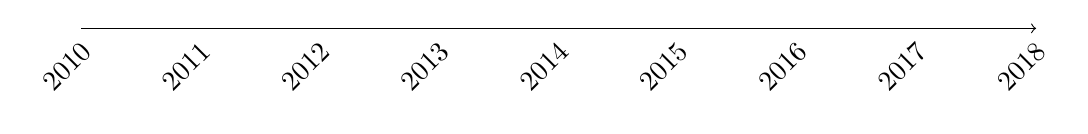
\begin{tikzpicture}
	\pgfmathtruncatemacro\start{2010} %Start year
	\pgfmathtruncatemacro\ende{2018}  %End year
	\pgfmathtruncatemacro\differenz{\ende-\start}
	
	\draw[->](0,0) -- (\textwidth, 0);
	\foreach \j in {0,..., \differenz} {
	    \pgfmathsetlengthmacro\tmp{\j*\textwidth/\differenz}
	    \pgfmathtruncatemacro\jahr{\start+\j}
	    \draw (\tmp,0) node[rotate=45, left, yshift=-6pt] {\jahr};
	}
\end{tikzpicture}
\end{document}